\documentclass[11pt]{article}
\usepackage[T1]{fontenc}
\usepackage[utf8]{inputenc}
\usepackage{lmodern,amsmath,amssymb,amsthm,mathtools}
\input{glyphtounicode.tex}
\input{glyphtounicode-cmex.tex}
\ifdefined\pdfglyphtounicode
\pdfglyphtounicode{tfm:rm-lmr10/Delta}{0394}
\pdfglyphtounicode{tfm:rm-lmr8/Delta}{0394}
\pdfglyphtounicode{tfm:lmsy10/E}{2130}
\pdfglyphtounicode{tfm:lmsy10/K}{1D4A6}
\pdfglyphtounicode{tfm:lmsy10/L}{2112}
\pdfglyphtounicode{tfm:lmsy8/E}{2130}
\pdfglyphtounicode{tfm:msbm10/E}{1D53C}
\pdfglyphtounicode{tfm:msbm10/P}{2119}
\pdfglyphtounicode{tfm:msbm10/R}{211D}
\pdfglyphtounicode{tfm:msbm10/T}{1D54B}
\pdfglyphtounicode{tfm:msbm10/Z}{2124}
\pdfglyphtounicode{tfm:lmsy10/bardbl}{2016}
\pdfglyphtounicode{tfm:lmsy10/backslash}{2216}
\pdfglyphtounicode{tfm:lmsy8/backslash}{2216}
\pdfglyphtounicode{tfm:lmex10/vextenddouble}{2016}
\pdfglyphtounicode{tfm:lmex10/parenleftbig}{0028}
\pdfglyphtounicode{tfm:lmex10/parenrightbig}{0029}
\pdfglyphtounicode{tfm:lmex10/bracketleftbig}{005B}
\pdfglyphtounicode{tfm:lmex10/bracketrightbig}{005D}
\pdfglyphtounicode{tfm:lmex10/floorleftbig}{230A}
\pdfglyphtounicode{tfm:lmex10/floorrightbig}{230B}
\pdfglyphtounicode{tfm:lmex10/parenleftBig}{0028}
\pdfglyphtounicode{tfm:lmex10/parenrightBig}{0029}
\pdfglyphtounicode{tfm:lmex10/parenleftbigg}{0028}
\pdfglyphtounicode{tfm:lmex10/parenrightbigg}{0029}
\pdfglyphtounicode{tfm:lmex10/bracketleftbigg}{005B}
\pdfglyphtounicode{tfm:lmex10/bracketrightbigg}{005D}
\pdfglyphtounicode{tfm:lmex10/floorleftbigg}{230A}
\pdfglyphtounicode{tfm:lmex10/floorrightbigg}{230B}
\pdfglyphtounicode{tfm:lmex10/parenleftBigg}{0028}
\pdfglyphtounicode{tfm:lmex10/parenrightBigg}{0029}
\pdfglyphtounicode{tfm:lmex10/braceleftBigg}{007B}
\pdfglyphtounicode{tfm:lmex10/summationtext}{2211}
\pdfglyphtounicode{tfm:lmex10/producttext}{220F}
\pdfglyphtounicode{tfm:lmex10/intersectiontext}{22C2}
\pdfglyphtounicode{tfm:lmex10/summationdisplay}{2211}
\pdfglyphtounicode{tfm:lmex10/productdisplay}{220F}
\pdfglyphtounicode{tfm:lmex10/tildewide}{02DC}
\pdfglyphtounicode{tfm:lmex10/ceilingleftBig}{2308}
\pdfglyphtounicode{tfm:lmex10/ceilingrightBig}{2309}
\pdfglyphtounicode{tfm:lmex10/radicalBig}{221A}
\fi
\pdfgentounicode=1
\usepackage[a4paper,margin=28mm]{geometry}
\usepackage{microtype,enumitem,booktabs,graphicx,xcolor}
\usepackage{needspace}
\usepackage{tikz}
\usetikzlibrary{arrows.meta,calc,positioning}
\usepackage{xurl}
\usepackage[colorlinks=true,linkcolor=blue!45!black,citecolor=blue!45!black,urlcolor=blue!45!black]{hyperref}
\usepackage[nameinlink,capitalise,noabbrev]{cleveref}
\newtheorem{theorem}{Theorem}[section]
\newtheorem{lemma}[theorem]{Lemma}
\newtheorem{proposition}[theorem]{Proposition}
\newtheorem{corollary}[theorem]{Corollary}
\theoremstyle{definition}
\newtheorem{definition}[theorem]{Definition}
\theoremstyle{remark}
\newtheorem{remark}[theorem]{Remark}
\newcommand{\Z}{\mathbb Z}
\newcommand{\R}{\mathbb R}
\newcommand{\T}{\mathbb T}
\newcommand{\N}{\mathbb N}
\newcommand{\Pp}{\mathbb P}
\newcommand{\E}{\mathbb E}
\newcommand{\norm}[1]{\left\lVert#1\right\rVert}
\newcommand{\dist}{\operatorname{dist}}
\newcommand{\floor}[1]{\left\lfloor#1\right\rfloor}
\newcommand{\ceil}[1]{\left\lceil#1\right\rceil}
\newcommand{\cO}{\mathcal O}
\newcommand{\cU}{\mathcal U}
\newcommand{\cV}{\mathcal V}
\newcommand{\cL}{\mathcal L}
\newcommand{\cK}{\mathcal K}
\newcommand{\cB}{\mathcal B}
\newcommand{\eps}{\varepsilon}
\newcommand{\id}{\mathrm{id}}
\DeclareMathOperator{\lcm}{lcm}
\setlist{itemsep=2pt,topsep=5pt}
\numberwithin{equation}{section}
\hypersetup{pdfauthor={OpenAI},pdftitle={Quantitative Superexponential Bounds for van der Waerden Numbers}}

\title{Quantitative Superexponential Bounds\\for van der Waerden Numbers}
\author{OpenAI}
\date{September 23, 2026}
\begin{document}
\maketitle
\begin{abstract}
We prove that there are absolute constants $c>0$ and $K_0$ such that
$W_r(k)>k^{ck\lfloor\log_2 r\rfloor}$ for every $k\ge K_0$ and $r\ge2$.
Consequently $W_r(k)^{1/k}\to\infty$ for each fixed $r\ge2$, giving a
quantitative positive resolution of Erd\H{o}s's superexponential-growth
question, including the two-color case.
\end{abstract}
\section{Introduction}
\label{sec:introduction}

For positive integers $r$ and $k$, let $W_r(k)$ be the least positive
integer $N$ such that every map $[N]\to[r]$ is constant on some
arithmetic progression
\[
 a,a+d,\ldots,a+(k-1)d,\qquad a,d\ge1,\quad a+(k-1)d\le N.
\]
Here $[N]=\{1,\ldots,N\}$, and using fewer than $r$ colors is allowed.
The finiteness of these numbers is van der Waerden's theorem
\cite{vanDerWaerden1927}.
The lower-bound problem asks how long an interval can be colored while
avoiding a monochromatic progression of a prescribed length. We prove
a bound with one threshold on the length, valid for every number of
colors.

\begin{theorem}
\label{main:intro}
There is an absolute integer $K_0$ such that, for every integer
$k\ge K_0$ and every integer $r\ge2$,
\[
 W_r(k)>k^{c k\lfloor\log_2r\rfloor},
 \qquad c=10^{-5}.
\]
\end{theorem}

In particular, for each fixed $r\ge2$,
\[
 \lim_{k\to\infty}W_r(k)^{1/k}=\infty.
\]
Erd\H{o}s explicitly asked for this full limit in the two-color case
\cite[p.~90, (2)]{erdos1980}.
Thus Theorem~\ref{main:intro} gives a quantitative positive resolution
of his superexponential-growth question.
It is stronger than the assertion that $W_2(k)/2^k$ tends to infinity.

\paragraph{Earlier bounds.}
Early lower bounds were obtained by Erd\H{o}s and Rado
\cite{erdosRado1952} and by Schmidt~\cite{schmidt1962}.
Berlekamp's algebraic construction gives
$W_2(p+1)>p2^p$ for every prime $p$ \cite[Theorem~2]{berlekamp1968}.
The local lemma of Erd\H{o}s and Lov\'asz~\cite{erdosLovasz1975}
provided another route to strong coloring bounds.
Szab\'o~\cite[Theorem~2]{szabo1990} proved
$W_2(k)\ge 2^k/k^\varepsilon$ for every fixed $\varepsilon>0$
and all sufficiently large $k$.
Kozik and Shabanov~\cite[Theorem~2]{kozikShabanov2016}
subsequently obtained an absolute $\beta>0$ such that
$W_r(k)\ge\beta r^{k-1}$ for all $r\ge2$ and $k\ge3$.
Hunter~\cite[Theorem~1]{hunter2025} improved the exponential base
for each fixed $r\ge5$, with a threshold allowed to depend on $r$.

Recent results distinguish the two questions posed by Erd\H{o}s.
Fox and Hunter \cite[Theorem~1]{foxHunter2026} proved
$W_3(k)>2^{k\log^*k/4}$ for all sufficiently large $k$, where
$\log^*k$ counts the iterations of the natural logarithm needed to
reach a value at most one.
Campos, Fox, and Schildkraut \cite[Theorem~1]{camposFoxSchildkraut2026}
proved
\[
 W_2(k)\ge(1-o(1))k2^{k-1}.
\]
They credit ChatGPT 5.6 Sol Pro with the coloring and an initial proof.
Their result settles the question about $W_2(k)/2^k$, whereas
Theorem~\ref{main:intro} gives the full superexponential limit.
For every fixed $\varepsilon\in(0,1)$, Fox and Hunter also prove
$W_r(k)\ge r^{(1-\varepsilon)k\log k}$ when $k$ is sufficiently
large in terms of $\varepsilon$ and
$r\ge(\log k)^{3/\varepsilon}$ \cite[Theorem~2]{foxHunter2026}.
For example, taking $\varepsilon=1/2$ gives a stronger lower bound
when $r\ge(\log k)^6$ and $k$ is sufficiently large. The bound here
holds uniformly down to two colors.

Growth in the number of colors, with the progression length fixed,
has a different history. Behrend's construction and Rankin's extension
to longer progressions supply dense progression-free sets
\cite{behrend1946,rankin1961}; covering an interval by translates of such
sets already gives superpolynomial growth in the number of colors
\cite[pp.~2--3]{foxHunter2026}. For three-term progressions, the density
bound of Kelley and Meka gives a quasipolynomial coloring upper bound
\cite[Theorems~1.1--1.2]{kelleyMeka2023}. For each fixed length at least
five, Leng, Sah, and Sawhney obtained further density bounds, improving
the earlier general coloring upper bounds
\cite[Theorem~1.1]{lengSahSawhney2024}.

For completeness, Theorem~\ref{transfer:large-r} gives a direct elementary
lower bound with an explicit constant uniform over all lengths $k\ge3$.
Combining it with the coloring upper bound in the
companion paper~\cite[Equation~(1.3)]{openaiArithmeticProgressions2026}
gives, for each integer $k\ge3$, a constant $A_k\ge1$ such that
for every integer $r\ge256$,
\[
 \exp\!\left(\frac{(\log r)^2}{64\log2}\right)
 <W_r(k)\le
 \left\lceil\exp\bigl(A_k(2+\log r)^{A_k}\bigr)\right\rceil.
\]
Thus, for every fixed progression length $k\ge3$, as integer $r$ tends
to infinity, growth in the number of colors is superpolynomial but at
most quasipolynomial: the lower
bound gives $W_r(k)/r^D\to\infty$ for every fixed real $D>0$, while
the upper bound has logarithm at most a fixed power of $\log r$.
The upper constant and exponent may depend on $k$; no uniform bound
on that dependence or matching logarithmic exponent is asserted.
Appendix~\ref{sec:upper} gives an elementary recursive upper bound,
including a proof of finiteness.
This is a coarse version of the classical argument; quantitative upper
bounds include Shelah's primitive-recursive bound~\cite{shelah1988}
and the bounds following from Gowers's proof of Szemer\'edi's
theorem~\cite{gowers2001}.
The boundary cases are $W_1(k)=k$, $W_r(1)=1$, and $W_r(2)=r+1$.

\paragraph{The construction and its quantitative ingredient.}
We first construct a two-coloring of a cyclic group $\Z/q^D\Z$ with
$q^D\ge k^{ck}$, where $q$ is a power of a prime exceeding $k$.
Let $\lambda$ be an integer dilation, to be chosen below.
The homomorphisms
\[
 x_i(n)=n/q^i\pmod1,\qquad y_i(n)=\lambda x_i(n),
 \qquad 1\le i\le D,
\]
supply two systems of circle coordinates.
Partition each coordinate circle into small intervals, and label a point
by the tuple of intervals containing its coordinates.
An outer color is assigned to each such label.
The intervals for $y$ become finer near the cut used to select real
representatives.
We arrange that every $k$-term cyclic progression with nonzero step
either contains a positive proportion of each outer color or has
globally affine real representatives in the $y$ coordinates.

A heavily repeated label determines a short rational period $h$.
The quantitative obstacle is to control such returns when the dimension
grows with $k$: constants depending arbitrarily on the dimension would
not suffice.
The quantitative choice is to let $D$ grow and to make $\lambda$
contain the full primary part, at every prime at most $D^2$, of
every possible period $h\le2\lceil k^{1/2}\rceil$.
After dilation, each scalar rational period is either one or exceeds
$D^2$.
This separation permits a local test on entire period blocks.
A key estimate counts the patterns through one specified label by
$(CDh)^{6D}$, with an absolute $C$ independent of $q$, $\lambda$,
and the width of the anchor interval.
It follows by anchoring at one visit and counting affine comparisons
in two scalar parameters at a time.
This form of counting remains useful even when some intervals are
arbitrarily small.

We attach an independent Bernoulli$(p)$ flip to each key consisting
of a $y$-box and $\lfloor\|q\widetilde y\|_2^2\rfloor$, where
$p=k^{-1/20}$ and $\widetilde y\in[-1/2,1/2)^D$ is the centered
representative. Here $\|\cdot\|_2$ is the Euclidean norm.
Every occurrence of a key uses the same flip, and each key occurs
at most four times along a progression.
Making a progression rich in both outer colors monochromatic
therefore requires many rare flips.
In the possibly overlapping affine case, monochromaticity prescribes
values for many distinct flip variables. The global label-word count,
together with the three coefficients of the quadratic squared norm,
gives only a small family of words of outer colors and actual keys;
identical words prescribe the same event.
With $D=\lceil k^{1/10}\rceil$, their logarithmic count is
$O(k^{9/10}\log k)=o(pk)$.
The two resulting probability estimates eliminate every progression.
A deterministic digit product then gives all $r\ge2$.

The squared-norm geometry continues the tradition of
Behrend's construction~\cite{behrend1946}; Green and Wolf
\cite{greenWolf2010} give a torus-annulus proof of Elkin's refinement.
For the asymmetric problem of excluding a red three-term progression
and a blue long progression, Green~\cite{green2022} uses translates
of a randomly perturbed ellipsoidal annulus, while
Hunter~\cite{hunter2022} chooses annulus radii independently at many centers.
Here the randomness is attached to coordinate boxes and integer
squared-norm bands. Least-common-multiple dilations in cyclic groups
appear in Fox and Hunter~\cite{foxHunter2026}; digit carry control and
finite-field norm colorings for a related symmetric-progression problem
appear in Shi and Dong~\cite{shiDong2026}.
We prove all geometric, counting, and probabilistic ingredients needed
here, including the finite local lemma.

\paragraph{Organization.}
Section~\ref{sec:setup} fixes the cyclic group and the two meshes.
Section~\ref{sec:counting} proves the global and anchored pattern counts,
and Section~\ref{sec:outer} uses them to construct the outer coloring.
Section~\ref{sec:dichotomy} turns its local tests into the balanced-or-affine
alternative. Section~\ref{perturb:section} introduces the norm-indexed
perturbation and proves the cyclic two-color theorem.
Section~\ref{sec:transfers} transfers that theorem to integer intervals
and all color counts, and proves the additional growth statements.
Appendix~\ref{sec:upper} supplies the elementary finite upper bound.

\section{The cyclic model and its coordinate meshes}\label{sec:setup}

We now choose the cyclic group and the two coordinate partitions on
which the two-color construction will be built.
All logarithms without an indicated base are natural. Throughout the cyclic
construction, $k$ is an integer exceeding an absolute threshold. Every
constant implicit in $O(\cdot)$ is absolute unless an explicit subscript
indicates otherwise, and every limiting assertion is as $k\to\infty$.
In particular, no threshold in the construction depends on the eventual
number of colors $r$.

Set
\begin{equation}\label{setup:parameters}
\begin{gathered}
 c=10^{-5},\qquad \delta=\frac1{10},\qquad \gamma=\frac1{100},\qquad
 D=\ceil{k^{1/10}},\qquad M=\ceil{k^{1/2}},\\
 h_0=D^2,\qquad p=k^{-1/20},\qquad H=k^{-2},\qquad
 \eta=\frac1{1000D}.
\end{gathered}
\end{equation}
We take $k$ large enough that $h_0<2M<k$.
The parameter $p$ will be the probability of a later perturbation. The
integer dilation
\begin{equation}\label{setup:dilation-definition}
 \lambda=\prod_{\substack{\ell\le h_0\\ \ell\text{ prime}}}
 \ell^{\floor{\log(2M)/\log\ell}}
\end{equation}
removes the small prime factors of all periods at most $2M$.
Least-common-multiple dilations also occur in the cyclic constructions
of Fox and Hunter~\cite{foxHunter2026}. The primary-factor choice here
is tailored to the growing dimension, as the next lemma records.

\begin{lemma}[Dilation of short periods]\label{setup:dilation}
We have $\log\lambda\le h_0\log(2M)$. If $1\le h\le2M$, then
every prime-power divisor of $h$ with prime at most $h_0$ divides
$\lambda$. Consequently, $h\mid\lambda$ whenever $h\le h_0$, and, for
every integer $t$, the denominator
\begin{equation}\label{setup:denominator}
 s=\frac{h}{\gcd(h,\lambda t)}
\end{equation}
is either $1$ or greater than $h_0$.
\end{lemma}

\begin{proof}
Each factor in \Cref{setup:dilation-definition} is at most $2M$,
and there are at most $h_0$ factors. If $\ell^a\mid h\le2M$, with
$\ell\le h_0$, then $a\le\floor{\log(2M)/\log\ell}$.
Thus the full $\ell$-primary part of $h$ divides $\lambda$, and hence
also $\gcd(h,\lambda t)$. All prime divisors of $s$ therefore exceed
$h_0$. This proves the assertions, including the case $t=0$, for which
$s=1$.
\end{proof}

\begin{lemma}[An elementary prime bound]\label{setup:prime}
For all sufficiently large integers $k$, there is a prime $P$ satisfying
$k<P\le2k^2$.
\end{lemma}

\begin{proof}
Put $n=k^2$. For a prime $\ell$, write $v_\ell(a)$ for the exponent
of $\ell$ in a positive integer $a$. Counting multiples of each power
of $\ell$ in the factorials gives
\[
 v_\ell\binom{2n}{n}
 =\sum_{a\ge1}\left(\floor{\frac{2n}{\ell^a}}
              -2\floor{\frac n{\ell^a}}\right)
 \le\floor{\log_\ell(2n)},
\]
because each summand is $0$ or $1$ and vanishes for $\ell^a>2n$.
If every prime factor of $\binom{2n}{n}$ were at most $k$, its value
would consequently be at most $(2n)^k$. On the other hand, the central
binomial coefficient is the largest of the $2n+1$ coefficients in
$(1+1)^{2n}$, so
\[
 \binom{2n}{n}\ge\frac{4^n}{2n+1}.
\]
For $n=k^2$, the logarithm of this lower bound is
$k^2\log4-\log(2k^2+1)$, whereas that of $(2n)^k$ is
$k\log(2k^2)$. The former is larger for all sufficiently large $k$.
There is therefore a prime divisor $P>k$; it is at most $2n$ because it
divides $(2n)!$.
\end{proof}

Choose such a prime $P$, and let $q$ be the least power of $P$ that is
at least $k^{ck/D}$. Minimality gives
\begin{equation}\label{setup:q-bounds}
 k^{ck/D}\le q\le2k^2 k^{ck/D},\qquad
 ck\log k\le D\log q\le ck\log k+D\log(2k^2).
\end{equation}
Here $q$ is a prime power, and need not itself be prime. Since
$h_0<k<P$ for large $k$, \Cref{setup:dilation-definition} shows that
$\gcd(\lambda,q)=1$. Define the remaining scales by
\begin{equation}\label{setup:mesh-parameters}
 H_x=\frac H\lambda,\qquad \alpha=q^{-(D+1)}.
\end{equation}
The parameter estimates used below include
\begin{equation}\label{setup:orders}
 D=O(k^{1/10}),\quad M=O(k^{1/2}),\quad
 \log\lambda=O(k^{1/5}\log k),\quad
 \log q=O(k^{9/10}\log k).
\end{equation}
These follow directly from \Cref{setup:parameters,setup:dilation,setup:q-bounds}.

Write $N=q^D$ and $G=\Z/N\Z$. We seek a two-coloring of $G$ with no
monochromatic progression
\begin{equation}\label{setup:cyclic}
 n_j=n_0+jd\quad(0\le j<k),\qquad n_0,d\in G,\qquad d\ne0.
\end{equation}
Every nonzero element of this prime-power cyclic group has order at
least $P>k$, so the $k$ displayed terms are distinct. On the circle
$\T=\R/\Z$, equipped with its usual distance and circumference one,
use the homomorphisms
\begin{equation}\label{setup:coordinates}
 x_i(n)=\frac n{q^i}\pmod1,\qquad
 y_i(n)=\lambda x_i(n)\qquad(1\le i\le D).
\end{equation}
They are well defined on $G$ since $q^i\mid N$. Write
$x(n)=(x_i(n))_{i=1}^D$ and $y(n)=(y_i(n))_{i=1}^D$, and fix their
representatives
\[
 \hat x(n)\in[0,1)^D,\qquad \tilde y(n)\in[-1/2,1/2)^D.
\]
The first coordinates will distinguish residue classes of a rational
return period. The dilation in the second coordinates removes rational
motion for periods at most $h_0$; the mesh near their representative
cut will then allow us to prove a global affine lift in that case.
The cut for the second representative system is the circle point
$1/2=-1/2$. Its distance function is
\begin{equation}\label{setup:cut-distance}
 \rho(Y)=\dist_{\T}(Y,1/2).
\end{equation}
Thus $0\le\rho\le1/2$, and $\rho$ is $1$-Lipschitz.

The first partition, denoted $U$, consists of the intervals
\[
 [aH_x,(a+1)H_x),\qquad 0\le a<k^2\lambda.
\]
This is an exact partition of $[0,1)$ because $H_x^{-1}=k^2\lambda$
is integral. The second partition becomes finer near its cut.
The positive scale $\alpha$ keeps this mesh finite; its choice will
be compared with the discrete step lattice in the short-period
argument of \Cref{dichotomy:main}. Put
\begin{equation}\label{mesh:definition}
 R=\log\left(1+\frac1{2\alpha}\right),\qquad
 m=\ceil{k^2R},\qquad
 a_\ell=\alpha\bigl(e^{\ell R/m}-1\bigr)\quad(0\le\ell\le m).
\end{equation}
The partition $V$ of $[-1/2,1/2)$ consists of
\begin{equation}\label{mesh:intervals}
 [-1/2+a_\ell,-1/2+a_{\ell+1}),\qquad
 [1/2-a_{\ell+1},1/2-a_\ell)
 \quad(0\le\ell<m).
\end{equation}
Since $a_0=0$ and $a_m=1/2$, these $2m$ intervals partition the
representative interval. They assign zero to the interval on its
right and the cut to the interval beginning at $-1/2$.
The same intervals also denote their images in $\T$. Closures and
neighborhoods of intervals will be taken on the circle; $|I|$ denotes
arc length.

For a circle point, $U(X)$ or $V(Y)$ denotes its individual interval
label, with the half-open conventions above. The full-label space and
label maps are
\begin{equation}\label{setup:labels}
 \begin{split}
 \cL&=U^D\times V^D,\\
 L(X,Y)&=\bigl((U(X_i))_{i=1}^D,(V(Y_i))_{i=1}^D\bigr),\\
 L(n)&=L(x(n),y(n)).
 \end{split}
\end{equation}
In particular, the identity of a label specifies each interval itself,
including its location on the circle.

\Needspace{3\baselineskip}
\begin{lemma}[Widths of the adaptive mesh]\label{mesh:width}
For every $I\in V$ and every $Y\in\overline I$,
\begin{equation}\label{mesh:width-bounds}
 \frac14H\bigl(\rho(Y)+\alpha\bigr)
 \le |I|\le2H\bigl(\rho(Y)+\alpha\bigr)\le2H.
\end{equation}
Moreover, $|V|=2m=O(k^3\log k)$.
\end{lemma}

\begin{proof}
For large $k$ we have $\alpha\le1/4$ and $R\ge1$. If
$\theta=R/m$, the bounds $k^2R\le m\le k^2R+1\le2k^2R$ give
$H/2\le\theta\le H$. On either interval indexed by $\ell$ in
\Cref{mesh:intervals}, the quantity $\rho(Y)+\alpha$ ranges, on the
closure, between $b=\alpha e^{\ell\theta}$ and $be^\theta$, while
$|I|=b(e^\theta-1)$. Hence
\[
 1-e^{-\theta}\le\frac{|I|}{\rho(Y)+\alpha}\le e^\theta-1.
\]
For $0\le\theta\le1$, the outside expressions are bounded below by
$\theta/2$ and above by $2\theta$, respectively. This proves the
first two inequalities in \Cref{mesh:width-bounds}; the last follows
from $\rho(Y)+\alpha\le3/4<1$.
Finally,
\[
 R\le(D+1)\log q=O(k\log k)
\]
by \Cref{setup:q-bounds}, so $2m\le2k^2R+2=O(k^3\log k)$.
\end{proof}

\begin{lemma}[Uniform neighborhoods]\label{mesh:neighbors}
For $I\in V$, let $w=|I|$ and
\[
 N(I)=\{Y\in\T:\dist_{\T}(Y,\overline I)\le w\}.
\]
Every $J\in V$ whose closure meets $N(I)$ satisfies $|J|\ge w/16$.
The arc $N(I)$ contains at most $49$ mesh endpoints.
\end{lemma}

\begin{proof}
Fix $Y_0\in\overline I$ and put $r_0=\rho(Y_0)+\alpha$.
Every $Y\in N(I)$ has circle distance at most $2w$ from $Y_0$.
By \Cref{mesh:width} and the Lipschitz property of $\rho$,
\[
 \rho(Y)+\alpha\ge r_0-2w\ge(1-4H)r_0\ge r_0/2,
\]
where the last inequality holds for $H\le1/8$. Apply the lower width
bound at a point of $\overline J\cap N(I)$ to obtain
\[
 |J|\ge\frac18Hr_0\ge\frac{w}{16}.
\]
The arc $N(I)$ has length $3w<1$. In its linear ordering, successive
mesh endpoints enclose a full mesh interval, of length at least
$w/16$ by the assertion just proved. If there are $b$ such endpoints,
then $(b-1)w/16\le3w$, so $b\le49$.
\end{proof}

For local counting in rotating coordinates, we ignore the fine mesh
within distance $\eta$ of the cut. Define the truncated output by
\begin{equation}\label{mesh:truncation-definition}
 V_\eta(Y)=
 \begin{cases}
 V(Y),&\rho(Y)\ge\eta,\\
 *,&\rho(Y)<\eta,
 \end{cases}
\end{equation}
where $*$ is a symbol distinct from every interval label. In particular,
equality at the threshold gives the actual interval label.

\begin{lemma}[Local complexity after truncation]\label{mesh:truncated}
On every circle arc of length at most $4H$, the output $V_\eta$ is
constant between at most $16004D$ breakpoints. Its value at a
breakpoint is also determined, and need not equal either neighboring
value.
\end{lemma}

\begin{proof}
The portion of the arc on which $\rho\ge\eta$ has at most two
components. Within one component, successive mesh endpoints have
spacing at least $H\eta/4$, by \Cref{mesh:width} applied at either
endpoint of the intervening mesh interval. The number of mesh
endpoints in these components is therefore at most
$4H/(H\eta/4)+2=16/\eta+2$. Add the at most two threshold points
$\rho=\eta$. Inside $\{\rho<\eta\}$ the output is constant, so no
other endpoints are needed. This gives at most
$16/\eta+4=16000D+4\le16004D$ breakpoints. At each breakpoint use
the half-open convention for $V$ and the weak inequality in
\Cref{mesh:truncation-definition}; this includes coincident mesh and
threshold points.
\end{proof}

\section{Counting global words and anchored local patterns}\label{sec:counting}

All counts in this section are counts of literal interval labels.
The central observation is that each scalar coordinate can be counted
using an arrangement in two real parameters, even though the number
$D$ of coordinates grows with $k$.
We use the standard hyperplane-arrangement region count; see
Stanley~\cite[Lemma~2.1 and Proposition~2.4]{stanley2007}.
The elementary proof below also counts equality signs, which are needed
for the half-open mesh intervals.

\begin{lemma}[Affine comparisons, including equality]\label{count:arrangement}
Let $s$ affine hyperplanes be given in $\R^e$, and record, for each
hyperplane, the sign in $\{-,0,+\}$ of a defining affine function.
The number of realized joint sign vectors is at most
\begin{equation}\label{count:arrangement-bound}
 \sum_{d=0}^e\binom{s}{d}\sum_{j=0}^{e-d}\binom{s}{j}
 \le(e+1)^2(s+1)^e.
\end{equation}
The same bound applies when the parameter space is restricted to an
arbitrary subset of $\R^e$.
\end{lemma}

\begin{proof}
First count strict sign vectors. The complement of an arrangement
has at most $\sum_{j=0}^e\binom{s}{j}$ regions. Indeed, when a new
hyperplane is added, every region it splits meets that hyperplane in
a different region of the induced arrangement, whose dimension is
at most $e-1$. Induction on $s$ and $e$, followed by Pascal's identity,
gives the stated bound. Repeated hyperplanes create no additional
regions. A strict sign set is convex, and therefore connected when
nonempty, so each strict sign vector corresponds to one region.

Now consider a realized sign vector with zero entries, and let $A$
be the affine intersection of its zero hyperplanes. If $A$ has
codimension $d$, then $d$ of those equations with linearly independent
normals already define $A$: consistency at a point of $A$ makes every
remaining zero equation a consequence of the selected equations.
There are at most $\binom{s}{d}$ ways to select them. On $A$, every
hyperplane containing $A$ has forced zero sign; the remaining
hyperplanes impose strict signs in dimension $e-d$. The strict-region
bound on $A$, and a sum over $d$, prove the first inequality in
\Cref{count:arrangement-bound}. For each summand,
$\binom{s}{d}\binom{s}{j}\le(s+1)^{d+j}\le(s+1)^e$;
there are at most $(e+1)^2$ summands. Restricting the parameter space
can only remove sign vectors.
\end{proof}

\begin{lemma}[Global label words]\label{count:global}
Let $T_{\mathrm{glob}}$ be the number of words
$\bigl(L(n_j)\bigr)_{0\le j<k}$ arising from the progressions in
\Cref{setup:cyclic}. Then
\begin{equation}\label{count:global-bound}
 \log T_{\mathrm{glob}}
 =O\bigl(D(\log k+\log\lambda)\bigr)
 =O(k^{3/10}\log k)=o(M).
\end{equation}
\end{lemma}

\begin{proof}
Consider any circle partition with $F$ endpoints, including its
representative cut, and freely choose a scalar start and step
$a,b\in[0,1)$. For $0\le j<k$, the unreduced value $a+jb$ belongs
to $[0,k)$. Represent the partition endpoints by numbers
$\tau\in[0,1)$. The interval containing $(a+jb)\bmod1$ is determined
by its comparisons with all $\tau+z$ for $-1\le z\le k$.
The comparisons for all $j$ use at most $3k^2F$ lines in the
two parameters $a,b$. Equality signs give precisely the assigned
half-open labels, so \Cref{count:arrangement} bounds the number of
scalar words by $9(3k^2F+1)^2$.

Apply this bound separately in all $2D$ scalar coordinates, allowing
their starts and steps to vary independently. This enlarges the
collection of possible words, and is therefore an upper bound for
the actual coordinate homomorphisms. We can take
\[
 F=|U|+|V|=k^2\lambda+O(k^3\log k).
\]
Since $\lambda\ge1$, we have
$\log F=O(\log k+\log\lambda)$, and thus
\[
 T_{\mathrm{glob}}\le\bigl[9(3k^2F+1)^2\bigr]^{2D}.
\]
This proves the first bound in \Cref{count:global-bound} with an
absolute constant. The remaining bounds follow from
\Cref{setup:orders} and $M\ge k^{1/2}$.
\end{proof}

For the local patterns fix an integer $h$ with $h_0<h\le2M$ and
$t\in\{0,\ldots,h-1\}^D$. In coordinate $i$ let
\begin{equation}\label{count:coordinate-periods}
 s_i=\frac{h}{\gcd(h,\lambda t_i)}.
\end{equation}
Call that second-system coordinate \emph{stationary} if $s_i=1$, and
\emph{rotating} otherwise. By \Cref{setup:dilation}, a rotating
coordinate has $s_i>h_0$. These descriptions depend only on $h,t$.
Stationarity concerns the rational step and permits nonzero drift;
even a period $h>h_0$ may have only stationary second coordinates.

We now define an enlarged family of full return-period blocks whose
labels can be balanced before the outer coloring is chosen.
\Cref{sec:dichotomy} will verify membership for every actual full
block with $h>h_0$ containing a position whose full label occurs more
than $k/M$ times in the whole progression.

\begin{definition}[Eligible local patterns]\label{count:eligible}
Choose $x,y\in\T^D$ and $u,v\in\R^D$, and form
\begin{equation}\label{count:local-paths}
 X_z=x+\frac z h(t+u),\qquad
 Y_z=y+\frac z h(\lambda t+v)\qquad(0\le z<h)
 \quad\text{in }\T^D.
\end{equation}
A position $z$ is \emph{regular} if
$\rho(Y_{z,i})\ge\eta$ in every rotating coordinate; if there are
no rotating coordinates, every position is regular. Record
$L(X_z,Y_z)$ at a regular position and a dummy symbol $*$ otherwise.
The resulting word in $(\cL\cup\{*\})^h$ is \emph{eligible for
$h,t$} if it admits a realization satisfying all of the following:
\begin{enumerate}[label=\textup{(\roman*)}]
 \item At least $h/2$ positions are regular, and the full labels at
       those positions are pairwise distinct.
 \item $|u_i|\le H_x$ for every $i$, and $|v_i|\le H$ in every
       rotating coordinate.
 \item In every stationary coordinate $i$, one has
       $|v_i|\le |V(Y_{z,i})|$ at every regular position $z$.
\end{enumerate}
The recorded word is the pattern; different realizations of one word
do not define additional patterns.
\end{definition}

The stationary drift bound is relative to interval width because those
intervals may be arbitrarily fine. This is the condition that makes
the following count independent of the anchor's width.

\begin{lemma}[Local patterns through a specified label]\label{count:local}
There is an absolute constant $C$ such that, for every
$h_0<h\le2M$ and every full label $\beta\in\cL$, the number of pairs
consisting of $t\in\{0,\ldots,h-1\}^D$ and an eligible pattern for
$h,t$ containing $\beta$ is at most
\begin{equation}\label{count:local-bound}
 (CDh)^{6D}.
\end{equation}
The constant is independent of $q$, $\lambda$, $\beta$, and $D$.
\end{lemma}

\begin{proof}
Fix $t$ and a position $z_0$ at which the recorded pattern equals
$\beta$. That position is regular. In each scalar coordinate,
re-anchor the path at $z_0$: let $a$ be the real representative of
that coordinate at $z_0$, in the interval specified by $\beta$,
and let $b$ be its drift variable, either $u_i$ or $v_i$.
At a target position $z$, an unreduced representative is
\begin{equation}\label{count:anchored-scalar}
 a+\tau_z+\frac{z-z_0}{h}b,
 \qquad
 \tau_z=\frac{(z-z_0)t_i}{h}
 \quad\hbox{or}\quad
 \tau_z=\frac{(z-z_0)\lambda t_i}{h},
\end{equation}
as appropriate. The translation $\tau_z$ is fixed once $t,z_0,z,i$
are fixed. We retain only the restrictions on $a,b$ implied at the
anchor, since discarding other restrictions can only increase the
number of outputs. The following three cases bound this number.

\emph{First-system coordinates.} Here $a$ ranges over an interval of length
$H_x$ and $|b|\le H_x$. Since $|z-z_0|/h<1$, the target range
is contained in a fixed real interval of length at most $3H_x$.
The real lifts of $U$-endpoints form a lattice of spacing $H_x$,
so at most four endpoints meet this range.

\emph{Stationary second-system coordinates.} Write $I=V(Y_{z_0,i})$.
The retained drift bound is $|b|\le |I|$, by the restriction at
the regular anchor. Also $\lambda t_i/h$ is integral, so the
translation $\tau_z$ is integral. Modulo one every target belongs
to $N(I)$ from \Cref{mesh:neighbors}, and at most $49$ mesh endpoints
are relevant. The unreduced target range lies in an interval of
length at most $3|I|<1$, so each relevant circle endpoint has at
most one lift in that range.

\emph{Rotating second-system coordinates.} The anchor interval has
width at most $2H$ and the retained drift bound is $|b|\le H$.
The target range has length at most $4H<1$. Apply
\Cref{mesh:truncated} to its image on the circle: at most $16004D$
breakpoints determine the truncated output $V_\eta$. Again each
circle breakpoint has at most one lift in the real target range.

In each case, the enclosing target interval and the finite list of
breakpoint lifts are fixed before $a,b$ are varied. In particular,
the magnitude of the fixed translation $\tau_z$ introduces no
factor in the count. Each comparison with a breakpoint lift is an
affine line in $(a,b)$. Taken over $0\le z<h$, there are at most
$16004Dh$ such lines per scalar coordinate. On the allowed parameter
rectangle, their signs determine the scalar output at every target.
They determine values at breakpoints as well as on open intervals;
this accounts for half-open endpoints and for exact equalities
$\rho=\eta$.

By \Cref{count:arrangement} with $e=2$, the number of possible scalar
output sequences is at most
\[
 9(16004Dh+1)^2\le C_0(Dh)^2
\]
for an absolute $C_0$. Take the product of these bounds for all $2D$
coordinates, truncating only rotating second-system coordinates.
Those scalar outputs determine the complete recorded pattern: a
position is dummy exactly when at least one rotating output is $*$;
at all other positions the outputs specify the full label. No
additional choice of a regular-position mask is needed.

There are $h^D$ choices of $t$ and at most $h$ choices of the anchor
$z_0$. Therefore the required number is at most
\[
 h^{D+1}\bigl[C_0(Dh)^2\bigr]^{2D}
 =C_0^{2D}D^{4D}h^{5D+1}
 \le(CDh)^{6D},
\]
where the last inequality holds for an absolute $C$, since $D\ge1$.
All eligible patterns containing $\beta$ have at least one such
anchor and are included in this count.
\end{proof}

\section{An outer coloring of the labels}
\label{sec:outer}

The pattern counts allow one coloring of $\cL$ to balance all the
tests needed below. For a fixed cyclic progression as in
\Cref{setup:cyclic}, call a full label \emph{light} if its multiplicity
in the progression is at most $k/M$, and \emph{heavy} otherwise.
A position has the same designation as its label. These designations
always refer to the whole progression, even when we later examine a
short block of its positions.

We first give the probabilistic tool, in its finite asymmetric form.
For the origins of the local lemma, see Erd\H{o}s and
Lov\'asz~\cite{erdosLovasz1975}; the proof of the form used here is included.

\begin{lemma}[Finite asymmetric local lemma]\label{outer:lll}
Let $\mathcal E$ be a finite family of events. Suppose a graph on
$\mathcal E$, with neighbor sets $\Gamma(E)$, has the property that each
$E$ is independent of the sigma-algebra generated by the events outside
$\{E\}\cup\Gamma(E)$. If numbers $z_E\in(0,1)$ satisfy
\begin{equation}\label{outer:lll-condition}
 \Pp(E)\le z_E\prod_{F\in\Gamma(E)}(1-z_F)
 \qquad(E\in\mathcal E),
\end{equation}
then $\Pp(\bigcap_{E\in\mathcal E}E^c)>0$.
\end{lemma}

\begin{proof}
For $T\subseteq\mathcal E$, write $A_T=\bigcap_{F\in T}F^c$.
We prove simultaneously, by induction on $|T|$, that
\begin{equation}\label{outer:conditional}
 \Pp(A_T)>0,
 \qquad
 \Pp(E\mid A_T)\le z_E\quad\text{for every }E\notin T.
\end{equation}
For $T=\varnothing$, positivity is immediate and the conditional bound
follows from \Cref{outer:lll-condition}. Suppose the assertions are
known for smaller sets. Removing any $F\in T$ and applying the
conditional bound gives
\[
 \Pp(A_T)=\Pp(A_{T\setminus\{F\}})
 \bigl(1-\Pp(F\mid A_{T\setminus\{F\}})\bigr)>0.
\]
To prove the conditional bound for $E\notin T$, put
$T_1=T\cap\Gamma(E)$ and $T_2=T\setminus T_1$.
If $T_1=\varnothing$, independence gives
$\Pp(E\mid A_T)=\Pp(E)\le z_E$ directly.
Otherwise, order the members of $T_1$ and condition successively on
their complements, starting with $A_{T_2}$. Each conditioning set has
size at most $|T|-1$, so the induction hypothesis yields
\[
 \Pp(A_{T_1}\mid A_{T_2})
 \ge\prod_{F\in T_1}(1-z_F).
\]
Using independence from $T_2$ in the numerator, we obtain
\[
 \Pp(E\mid A_T)
 \le\frac{\Pp(E\mid A_{T_2})}
             {\Pp(A_{T_1}\mid A_{T_2})}
 \le\frac{\Pp(E)}{\prod_{F\in T_1}(1-z_F)}
 \le z_E.
\]
The last inequality uses \Cref{outer:lll-condition} and
$T_1\subseteq\Gamma(E)$. This completes the induction; take
$T=\mathcal E$ for the conclusion.
\end{proof}

\begin{proposition}[Balanced outer coloring]\label{outer:coloring}
For all sufficiently large $k$, there is a map
$c_*:\cL\to\{0,1\}$ with the following properties.
\begin{enumerate}[label=\textup{(\roman*)}]
 \item In every cyclic progression having at least $\delta k$ light
 positions, each bit occurs on at least one quarter of its light
 positions when labels are colored by $c_*$.
 \item In every eligible recorded pattern of \Cref{count:eligible},
 each bit occurs on at least one quarter of its regular positions.
\end{enumerate}
The threshold on $k$ is absolute.
\end{proposition}

\begin{proof}
Assign to every $\beta\in\cL$ an independent uniform random bit
$\xi_\beta$. We introduce two finite families of bad events.

For the first family, take each distinct full-label word of a cyclic
progression with $L_0\ge\delta k$ light positions. Let $w_{\max}$
be the largest multiplicity of a light label. Order the light positions
by grouping equal labels together, with all choices fixed as functions
of the word. Distribute the resulting list cyclically among
$w_{\max}$ rows. A group has at most $w_{\max}$ positions, so a label
occurs at most once in each row. Every row has at least
\begin{equation}\label{outer:row-size}
 \floor{\frac{L_0}{w_{\max}}}
 \ge\delta M-1
\end{equation}
positions, because $w_{\max}\le k/M$.
For each row let its bad event be that some bit occurs on strictly
fewer than one quarter of its positions. There are at most
$kT_{\mathrm{glob}}$ such events in total, where
$T_{\mathrm{glob}}$ is the number in \Cref{count:global}.

For the second family, take one event for each eligible recorded
pattern and its discrete parameters $h,t$, where $h_0<h\le2M$.
Its bad event is that some bit occurs on strictly fewer than one
quarter of the regular positions. The tested labels are pairwise
distinct by eligibility, and their number is at least $h/2$.
Dummy positions use no variables. Although the realizations of the
patterns have real parameters, these event families are finite:
$\cL$, the word lengths, and the choices of $h,t$ are all finite.

Each event $E$ thus tests $l(E)$ distinct independent label variables.
If $X$ is the number of ones among $l=l(E)$ such variables, then
\[
 \E e^{\pm(X-l/2)}=(\cosh(1/2))^l\le e^{l/8}.
\]
Indeed, $(2j)!\ge2^j j!$ gives
$\cosh t\le e^{t^2/2}$ by termwise comparison of the power series.
Markov's inequality for the two deviations from $l/2$ consequently gives
\begin{equation}\label{outer:tail}
 \Pp(E)
 \le\Pp(X-l/2\le-l/4)+\Pp(X-l/2\ge l/4)
 \le2e^{-l(E)/8}.
\end{equation}
The weak tail inequalities also cover the strict inequalities defining
the bad events, regardless of divisibility of $l$ by four.

Give $E$ the weight $z_E=e^{-l(E)/32}$. By
\Cref{count:global,outer:row-size}, the total weight of all
first-family events is at most
\begin{equation}\label{outer:first-weight}
 kT_{\mathrm{glob}}e^{-(\delta M-1)/32}=o(1).
\end{equation}
For a fixed label $\beta$, \Cref{count:local} bounds the second-family
weight of events using $\xi_\beta$ by
\begin{equation}\label{outer:second-weight}
 \sum_{h_0<h\le2M}(CDh)^{6D}e^{-h/64}
 \le\sum_{h>D^2}(CDh)^{6D}e^{-h/64}=o(1).
\end{equation}
To see the last estimate uniformly, take $C\ge1$. The function
$\log(CDh)/h$ is decreasing for $h\ge D^2$ once $D$ is large,
and hence
\[
 \sup_{h>D^2}\frac{6D\log(CDh)}{h}
 \le\frac{6\log(CD^3)}{D}=o(1).
\]
For all sufficiently large $k$, each summand in the infinite sum in
\Cref{outer:second-weight} is therefore at most $e^{-h/128}$.
Its tail tends to zero as $D\to\infty$.

It follows from \Cref{outer:first-weight,outer:second-weight} that,
uniformly over all labels $\beta$,
\begin{equation}\label{outer:incident-weight}
 \sum_{E:\,\xi_\beta\text{ is used by }E}z_E\le\frac1{500}
\end{equation}
for all sufficiently large $k$. Join two distinct events whenever
their supports share a label variable. Since all label bits are
independent, this is a dependency graph of the kind required in
\Cref{outer:lll}; independence holds from the joint sigma-algebra of
all nonneighbors. By summing \Cref{outer:incident-weight} over the
$l(E)$ labels used by $E$, we have
\[
 \sum_{F\in\Gamma(E)}z_F\le\frac{l(E)}{500}.
\]
The lower bounds $l(E)\ge\delta M-1$ in the first family and
$l(E)\ge h/2>D^2/2$ in the second ensure that $l(E)\ge100$
eventually. In particular $z_E<1/2$. Since
$\log(1-z)\ge-2z$ for $0\le z\le1/2$, we obtain
\begin{align}
 z_E\prod_{F\in\Gamma(E)}(1-z_F)
 &\ge\exp\!\left[-\left(\frac1{32}+\frac2{500}\right)l(E)\right]
 \notag\\
 &\ge2e^{-l(E)/8}\ge\Pp(E).
 \label{outer:criterion}
\end{align}
For the second inequality, the positive difference
$1/8-1/32-2/500$ multiplied by $100$ exceeds $\log2$.
Thus \Cref{outer:lll} gives a choice of all label bits avoiding every
bad event. Fix that choice as $c_*$. Summing the balanced row counts
over the partition of the light positions proves part~\textup{(i)};
the second event family gives part~\textup{(ii)}.
All estimates used absolute constants and depended only on $k$, so
the threshold is absolute.
\end{proof}

Fix such a coloring from now on, and define its pullback to the group by
\begin{equation}\label{outer:pullback}
 c_0(n)=c_*(L(n))\qquad(n\in G).
\end{equation}

\section{Repeated labels and the outer-color dichotomy}
\label{sec:dichotomy}

We show that every cyclic progression either receives many occurrences
of each outer bit or admits one affine lift in the centered second
coordinates. The issue is repeated labels: a closest return to a heavy
label identifies a rational period and a small drift. Short periods
disappear under the dilation, while longer periods supply the eligible
patterns tested in \Cref{outer:coloring}.

\begin{lemma}[Affinity inside a small box]\label{dichotomy:affinity}
Let $z_j=a+jb$ in $\T^e$, for $0\le j<k$, and let
$J\subseteq\{0,\ldots,k-1\}$. Suppose real representatives
$Z_j\in\R^e$, $j\in J$, lie in one box whose coordinate intervals
have length at most $2H$. If $2kH<1$, there are $A,B\in\R^e$
such that $Z_j=A+jB$ for every $j\in J$.
\end{lemma}

\begin{proof}
For any $j_1<j_2<j_3$ in $J$, affinity modulo one implies that
\[
 (j_3-j_2)(Z_{j_2}-Z_{j_1})
 -(j_2-j_1)(Z_{j_3}-Z_{j_2})\in\Z^e.
\]
In each coordinate its absolute value is at most
$2H(j_3-j_1)\le2kH<1$, so it is zero. Thus every triple has the
same affine interpolation. If $|J|\ge2$, interpolate between its
smallest and largest indices to obtain $A,B$; the triple identity
places every remaining point on that interpolation. For at most two
indices the conclusion follows directly, including the empty case.
\end{proof}

Fix a cyclic progression $n_j=n_0+jd$, $0\le j<k$, with a heavy
label. In the next three lemmas the terms \emph{light} and \emph{heavy}
refer to this fixed progression.

\begin{lemma}[Closest return and drift]\label{dichotomy:drift}
Choose a heavy label and let $J$ be its set of occurrence indices,
with $m_*=|J|>k/M$. Let $h$ be the smallest positive difference
between two members of $J$, attained at $j'$ and $j'+h$.
Set
\[
 u=\hat x(n_{j'+h})-\hat x(n_{j'}),\qquad
 v=\tilde y(n_{j'+h})-\tilde y(n_{j'}).
\]
Then, for sufficiently large $k$,
\begin{equation}\label{dichotomy:drift-bounds}
 \begin{gathered}
 1\le h\le2M,\\
 |u_i|\le\frac{H_x}{m_*-1}\le\frac{2MH_x}{k},\qquad
 |v_i|\le\frac{2H}{m_*-1}\le\frac{4MH}{k}
 \quad(1\le i\le D),
 \end{gathered}
\end{equation}
and $v=\lambda u$ as real vectors.
\end{lemma}

\begin{proof}
For large $k$, the inequality $m_*>k/M$ gives
$m_*-1\ge k/(2M)$. Write $j_-=\min J$ and $j_+=\max J$.
The smallest of the $m_*-1$ consecutive gaps in $J$ satisfies
\[
 h\le\frac{j_+-j_-}{m_*-1}\le\frac{k-1}{m_*-1}\le2M.
\]
All vectors $(\hat x(n_j),\tilde y(n_j))$, $j\in J$, lie in
one full-label box, whose coordinate widths are at most $2H$ by
\Cref{mesh:width}. By \Cref{dichotomy:affinity}, their differences
are proportional to differences of indices. In particular the
difference at the chosen gap $h$ is $h/(j_+-j_-)$ times the difference
between the two extreme visits. The latter has first-coordinate
absolute differences at most $H_x$ and second-coordinate absolute
differences at most $2H$. This proves \Cref{dichotomy:drift-bounds}.

The identity $y=\lambda x$ on the torus implies
$v-\lambda u\in\Z^D$. Since $\lambda H_x=H$,
\[
 |v_i-\lambda u_i|\le\frac{6MH}{k}<1
\]
for large $k$. Every coordinate of this integer vector is therefore
zero.
\end{proof}

\begin{lemma}[Rational path and separated residues]\label{dichotomy:path}
With $h,u,v$ as in \Cref{dichotomy:drift}, there is
$t\in\{0,\ldots,h-1\}^D$ such that
\begin{equation}\label{dichotomy:path-equations}
 \begin{aligned}
 x(n_j)&=x(n_0)+\frac jh(t+u),\\
 y(n_j)&=y(n_0)+\frac jh(\lambda t+v)
 \end{aligned}
 \qquad\text{in }\T^D\quad(0\le j<k).
\end{equation}
Moreover $\gcd(t_1,\ldots,t_D,h)=1$, and indices incongruent
modulo $h$ have distinct full labels. Consequently, all occurrences
of any one full label lie in a single residue class modulo $h$.
\end{lemma}

\begin{proof}
Since $h x(d)=u$ modulo $\Z^D$, the vector
$t'=h\hat x(d)-u$ is integral. Reduce it coordinatewise modulo
$h$ to obtain $t$. The first equality in
\Cref{dichotomy:path-equations} follows; multiplication by $\lambda$
and the real identity $v=\lambda u$ give the second.

Suppose an integer $e>1$ divides $h$ and every $t_i$. It also divides
every $t'_i$, because $t'-t\in h\Z^D$. Hence the torus
displacements from index $j'$ to index $j'+h/e$ are $u/e$ and
$v/e$ in the first and second systems. The vector
\[
 (\hat x(n_{j'}),\tilde y(n_{j'}))+\frac1e(u,v)
\]
is a convex combination of the representatives at $j'$ and $j'+h$.
Their common full-label box is a product of half-open real intervals
and is convex. This vector therefore lies in that same box and is
the chosen representative of the sample at $j'+h/e$.
It gives an additional visit to the label at a strictly smaller
positive gap $h/e$, a contradiction. This proves the gcd assertion.

The torus vector $t/h$ has order exactly $h$: if $h$ divides all
$a t_i$, the gcd assertion and B\'ezout's identity imply $h\mid a$.
Take any $j_1,j_2\in\{0,\ldots,k-1\}$ incongruent modulo $h$.
In at least one coordinate the rational displacement
$(j_1-j_2)t_i/h$ has circle distance at least
$1/h$ from zero. The drift in that coordinate has absolute value at
most
\[
 \frac{k|u_i|}{h}\le\frac{2MH_x}{h}\le\frac{2MH}{h}.
\]
By the triangle inequality on the circle the actual displacement has
distance at least
\[
 \frac{1-2MH}{h}\ge\frac{1-2MH}{2M}>H\ge H_x
\]
for sufficiently large $k$. Two samples in the same $U$ interval
have circle distance at most $H_x$, so these samples cannot have
the same full label.
\end{proof}

\begin{lemma}[Drift relative to every heavy interval]
\label{dichotomy:heavy-width}
For every heavy index $j_*$ of the fixed progression and each
$1\le i\le D$,
\begin{equation}\label{dichotomy:relative-width}
 |v_i|\le\frac{2M}{k}\,|V(y_i(n_{j_*}))|.
\end{equation}
The heavy label here need not be the one used to choose $h$.
\end{lemma}

\begin{proof}
Let the full label at $j_*$ have multiplicity $m'>k/M$, and let
$j_-$ and $j_+$ be its extreme occurrence indices. By
\Cref{dichotomy:path}, $j_+-j_-=a h$ for an integer
$m'-1\le a<k/h$. Set $L_i=|V(y_i(n_{j_*}))|$. The real
representative difference
\[
 \Delta_i=\tilde y_i(n_{j_+})-\tilde y_i(n_{j_-})
\]
has $|\Delta_i|\le L_i\le2H$. From
\Cref{dichotomy:path-equations}, it is congruent to $a v_i$
modulo one. On the other hand,
\[
 |a v_i|\le\frac{4MH}{h},\qquad
 |\Delta_i-a v_i|\le2H+\frac{4MH}{h}<1
\]
for large $k$. The integer $\Delta_i-a v_i$ is zero. Therefore
\[
 |v_i|\le\frac{L_i}{a}\le\frac{L_i}{m'-1}
 \le\frac{2M}{k}L_i,
\]
as claimed. This argument uses only the two endpoint representatives;
it requires no assertion about the intervening path across a cut.
\end{proof}

\begin{theorem}[Outer-color dichotomy]\label{dichotomy:main}
For every sufficiently large $k$, the coloring $c_0$ from
\Cref{outer:pullback} has the following property. Every cyclic
progression $n_j=n_0+jd$, $0\le j<k$, with $d\ne0$ in $G$,
satisfies at least one of these alternatives:
\begin{enumerate}[label=\textup{(\roman*)}]
 \item each bit occurs among $c_0(n_0),\ldots,c_0(n_{k-1})$
 at least $\gamma k$ times;
 \item there are $A,B\in\R^D$ such that
 $\tilde y(n_j)=A+jB$ for all $0\le j<k$.
\end{enumerate}
The threshold on $k$ is absolute.
\end{theorem}

\begin{proof}
If the progression has at least $\delta k$ light positions,
\Cref{outer:coloring}\textup{(i)} supplies at least
$\delta k/4\ge\gamma k$ occurrences of each bit. We may therefore
assume that fewer than $\delta k$ positions are light. There is a
heavy label, and \Cref{dichotomy:drift,dichotomy:path,dichotomy:heavy-width}
provide $h,t,u,v$ with all the properties proved above.

\paragraph{Short periods.}
Suppose $h\le h_0$. The definition of the dilation gives
$h\mid\lambda$. Thus the second path in
\Cref{dichotomy:path-equations} has real step $w=v/h$ modulo one,
because $\lambda t/h$ is integral. Its total coordinate motion satisfies
\begin{equation}\label{dichotomy:short-motion}
 k|w_i|\le\frac{4MH}{h}<\frac12
\end{equation}
for large $k$. The congruence $w_i=y_i(d)$ modulo one also gives
$w_i\in q^{-i}\Z$: a representative of $y_i(d)$ is an integral
multiple of $q^{-i}$, and adding an integer preserves this lattice.
In particular,
\begin{equation}\label{dichotomy:step-lattice}
 w_i\ne0\quad\Longrightarrow\quad
 |w_i|\ge q^{-i}\ge q^{-D}\ge\alpha.
\end{equation}

Consider the real segment
$\tilde y_i(n_0)+\tau w_i$, $0\le\tau\le k-1$.
If the sampled centered representatives fail to equal
$\tilde y(n_0)+jw$, some coordinate has $w_i\ne0$ and this closed
segment meets a cut point in $1/2+\Z$. The word \emph{closed}
includes a cut met at the initial or final sample, so both directions
of motion and exact cut hits are covered. Each sampled point is
then within real distance $k|w_i|$ of such a cut point, giving
$\rho(y_i(n_j))\le k|w_i|$ for every $j$.
By \Cref{mesh:width,dichotomy:step-lattice},
\[
 |V(y_i(n_j))|
 \le2H\bigl(\rho(y_i(n_j))+\alpha\bigr)
 \le2H(k+1)|w_i|<|w_i|.
\]
Yet \Cref{dichotomy:short-motion} implies that any two distinct
sampled points in this coordinate have circle distance
$|j-j'|\,|w_i|\ge|w_i|$: the entire real displacement is less
than one half. They cannot belong to a common $V$ interval of width
less than $|w_i|$. All full labels would therefore be distinct,
contradicting the heavy label. Hence every sampled representative
equals $\tilde y(n_0)+jw$, proving alternative~\textup{(ii)}.

\paragraph{Longer periods.}
Suppose $h_0<h\le2M$. Partition the first
$h\floor{k/h}$ indices into consecutive full blocks of length $h$;
the remaining block has fewer than $h$ indices. A full block starting
at $j_0$ has exactly the form in \Cref{count:eligible}, with starting
points $x(n_{j_0}),y(n_{j_0})$ and the same $h,t,u,v$.
We verify its regularity and, when it contains a heavy index,
every condition of eligibility.

For a rotating coordinate $i$, let
$s_i=h/\gcd(h,\lambda t_i)>h_0$. Without the drift, the $h$
values
\[
 y_i(n_{j_0})+\frac{z\lambda t_i}{h},\qquad0\le z<h,
\]
run through an equally spaced grid of $s_i$ circle points, each
exactly $h/s_i$ times. The actual value at $z$ is within
$|v_i|\le4MH/k<\eta$ of this grid value. If the actual position is
nonregular in this coordinate, its grid value is within $2\eta$
of the cut. An arc of length $4\eta$ contains at most
$4\eta s_i+1$ points of an $s_i$-point grid. This bound remains
valid when endpoints are included. Consequently the fraction of
positions excluded by this coordinate is at most
$4\eta+1/s_i$. A union bound over rotating coordinates shows that
the fraction of nonregular positions is at most
\begin{equation}\label{dichotomy:regular-fraction}
 D\left(4\eta+\frac1{h_0}\right)
 =\frac4{1000}+\frac1D<\frac12.
\end{equation}
Thus each full block has at least $h/2$ regular positions. All labels
within the block are distinct by \Cref{dichotomy:path}, since its
indices have distinct residues modulo $h$. Also
$|u_i|\le H_x$ and $|v_i|\le H$ for all $i$ by
\Cref{dichotomy:drift-bounds}, for sufficiently large $k$.

Now use any full block containing a heavy index $j_*$.
Fix a stationary coordinate $i$ and write
$I_*=V(y_i(n_{j_*}))$, $L_*=|I_*|$. Its rational step
$\lambda t_i/h$ is integral, so for every index $j$ in the block,
\[
 \dist_{\T}\bigl(y_i(n_j),y_i(n_{j_*})\bigr)
 \le\frac{|j-j_*|}{h}|v_i|
 \le|v_i|\le\frac{2M}{k}L_*.
\]
For large $k$ this places $y_i(n_j)$ in the circular
$L_*$-neighborhood of $\overline{I_*}$. Applying
\Cref{mesh:neighbors} with $I=I_*$ and
$J=V(y_i(n_j))$ gives
\[
 |V(y_i(n_j))|\ge\frac{L_*}{16}\ge|v_i|,
\]
where the final inequality uses $2M/k\le1/16$ and
\Cref{dichotomy:relative-width}. This holds at every block position,
in particular at each regular position as eligibility requires.
The heavy index $j_*$ need not itself be regular: it serves only to
provide the interval $I_*$ and the relative drift estimate.
The neighborhood statement uses closures, so a cut crossing or an
endpoint equality causes no change in this verification.

Every full block containing a heavy index is therefore eligible.
By \Cref{outer:coloring}\textup{(ii)} and
\Cref{dichotomy:regular-fraction}, it contributes at least $h/8$
occurrences of each bit. A full block not used in this way consists
entirely of light positions. Since fewer than $\delta k$ positions
are light in the entire progression, and fewer than $h$ positions
lie in the remainder, the used full blocks cover at least
\[
 k-h-\delta k\ge\frac45 k
\]
positions for sufficiently large $k$, using $h\le2M=o(k)$.
Each bit consequently occurs at least $k/10\ge\gamma k$ times.
This proves alternative~\textup{(i)} and completes the dichotomy.
All inequalities imposed only absolute lower bounds on $k$.
\end{proof}

\section{A sparse perturbation of the outer coloring}
\label{perturb:section}

Fix the outer coloring $c_*$ supplied by \Cref{outer:coloring}, and put
$c_0(n)=c_*(L(n))$.  All randomness used to construct $c_*$ has now been
resolved.  We shall introduce new independent bits indexed by geometric
keys.  A key will occur only a bounded number of times on any sampled
progression.  This allows a small flip probability to preserve the
progressions containing many of each outer color.  For progressions with
affine lifts, a separate count of the possible keys makes the same small
probability sufficient.

Retain the parameters and cyclic progressions from
\Cref{setup:parameters,setup:cyclic}.  For $n\in G$, define
\begin{equation}\label{perturb:keys}
 f(n)=\norm{q\tilde y(n)}_2^2,
 \qquad
 \kappa(n)=\left((V(y_i(n)))_{i=1}^D,\,\floor{f(n)}\right),
 \qquad
 \cK=\{\kappa(n):n\in G\}.
\end{equation}
Thus a key records a specific second-system box and a specific integer
squared-norm band.  Since $G$ is finite, so is $\cK$.
The next lemma uses a bounded-width version of the equal-norm geometry
in Behrend's construction~\cite{behrend1946}: a thin norm band has
short intersections with a line on either side of its nearest point
to the origin.

\begin{lemma}[Bounded multiplicity of a key]\label{perturb:multiplicity}
For every progression $n_j=n_0+jd$ in $G$ with $d\ne0$ and
$0\le j<k$, every key occurs at most four times among the $\kappa(n_j)$.
\end{lemma}

\begin{proof}
First fix a second-system box, and let $J$ be the indices whose centered
representatives lie in that box.  Every coordinate interval has width at
most $2H$, so \Cref{dichotomy:affinity} gives
\[
 \tilde y(n_j)=A+jB\qquad(j\in J)
\]
for suitable $A,B\in\R^D$.  The indices in $J$ need not be consecutive.
In particular, the points $q\tilde y(n_j)$ lie on an affine line when
$|J|\ge2$; when $|J|\le1$ the claimed multiplicity bound is immediate.

Any two distinct terms of the progression give points separated by
Euclidean distance at least one after this scaling.  To see this, the
terms are distinct by \Cref{setup:cyclic}, and $\lambda$ is a unit modulo
$q^D$.  Hence $\lambda(n_j-n_{j'})$ is a nonzero residue modulo $q^D$.
Choose an integer representative $z$ of this residue, and let
$a\in\{0,\ldots,D-1\}$ be the largest integer for which $q^a\mid z$.
Divisibility by $q^b$, for $b\le D$, is unchanged upon adding a multiple
of $q^D$, so this choice is intrinsic to the residue.  Write $z=q^a u$;
then $q\nmid u$.  In coordinate $a+1$ the circle displacement is
\[
 y_{a+1}(n_j)-y_{a+1}(n_{j'})=\frac{u}{q}\pmod1.
\]
The residue of $u$ modulo $q$ is one of $1,\ldots,q-1$, whose distance
from $0$ on the circle after division by $q$ is at least $1/q$.
This argument requires only $q\nmid u$; it does not require $u$ to be a
unit or $q$ to be prime.  The difference between any two real
representatives has absolute value at least their circle distance.
Consequently
\begin{equation}\label{perturb:separation}
 \norm{q\tilde y(n_j)-q\tilde y(n_{j'})}_2\ge1
 \qquad(j\ne j').
\end{equation}

If $|J|\ge2$, these separated points determine a nonconstant affine
line $\ell$.  Let $z_0$ be the point of $\ell$ closest to the origin,
and choose a unit vector $e$ along $\ell$.  Writing its points as
$z_0+te$, with $t\in\R$, gives
\[
 \norm{z_0+te}_2^2=t^2+C',\qquad C'=\norm{z_0}_2^2\ge0,
\]
because $z_0$ is orthogonal to $e$.  For a fixed integer $m\ge0$, the
band of the key is
\[
 m\le t^2+C'<m+1.
\]
If it is nonempty, then $m+1-C'>0$, and on the half-line $t\ge0$ it
is contained in the closed interval with endpoints
\[
 \sqrt{\max\{0,m-C'\}},\qquad \sqrt{m+1-C'}.
\]
The difference of the quantities under these square roots is at most
one.  For $0\le u\le v$, the inequality
$(\sqrt v-\sqrt u)^2\le v-u$ therefore shows that this interval has
length at most one.  Reflection gives the same bound on $t\le0$.
By \Cref{perturb:separation}, each of these intervals contains at most
two sampled points: three points in an interval of length at most one
would have total separation at least two.  Thus the key occurs at most
four times.  If the band reaches the nearest point $z_0$, counting
$t=0$ in both halves only enlarges this upper bound.  Replacing the
half-open band by closed intervals also covers equality at either
boundary, and the case of exactly two points needs no additional
argument.
\end{proof}

\begin{figure}[htbp]
 \centering
 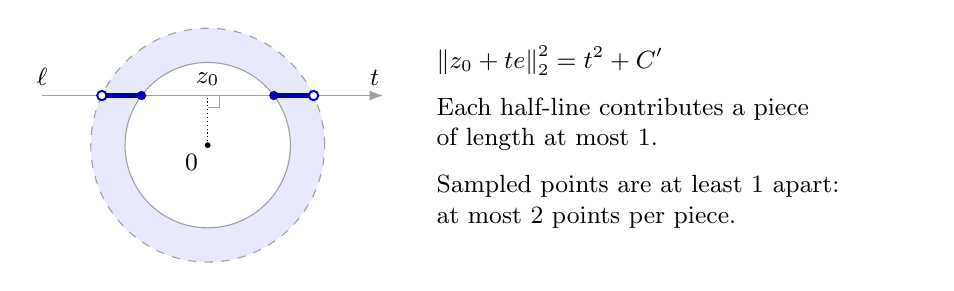
\begin{tikzpicture}[scale=1.05,>=Latex,
    every node/.style={font=\small}]
  \path[fill=blue!9,even odd rule]
    (0,0) circle[radius={sqrt(2)}] (0,0) circle[radius=1];
  \draw[gray!75] (0,0) circle[radius=1];
  \draw[gray!75,dashed] (0,0) circle[radius={sqrt(2)}];
  \draw[gray!75,->] (-2.0,0.6)--(2.12,0.6);
  \node[above left] at (-1.82,0.6) {$\ell$};
  \node[above] at (2.02,0.6) {$t$};
  \draw[blue!70!black,line width=2pt]
    ({-sqrt(1.64)},0.6)--(-0.8,0.6);
  \draw[blue!70!black,line width=2pt]
    (0.8,0.6)--({sqrt(1.64)},0.6);
  \fill[blue!70!black] (-0.8,0.6) circle[radius=1.6pt];
  \fill[blue!70!black] (0.8,0.6) circle[radius=1.6pt];
  \draw[blue!70!black,fill=white,line width=0.7pt]
    ({-sqrt(1.64)},0.6) circle[radius=1.6pt];
  \draw[blue!70!black,fill=white,line width=0.7pt]
    ({sqrt(1.64)},0.6) circle[radius=1.6pt];
  \draw[densely dotted] (0,0)--(0,0.6);
  \draw[gray!75] (0,0.46)--(0.14,0.46)--(0.14,0.6);
  \fill (0,0) circle[radius=1pt];
  \node[below left] at (0,0) {$0$};
  \node[above] at (0,0.6) {$z_0$};
  \node[align=left,anchor=west,text width=6.1cm] at (2.65,0.1)
    {$\norm{z_0+te}_2^2=t^2+C'$\par\medskip
     Each half-line contributes a piece\par
     of length at most $1$.\par\medskip
     Sampled points are at least $1$ apart:\par
     at most $2$ points per piece.};
\end{tikzpicture}

 \caption{A line meeting the band $m\le\norm{z}_2^2<m+1$, illustrated
 for $m=1$.  Solid endpoints belong to the inner boundary; open endpoints
 lie on the excluded outer boundary.  In general each half-line from
 the nearest point $z_0$ contributes length at most one, giving the
 four-point bound in \Cref{perturb:multiplicity}.}
 \label{perturb:norm-band}
\end{figure}

Call a cyclic progression \emph{affine} when its entire sequence of
centered representatives $\tilde y(n_j)$ is affine in $j$ as a sequence
in $\R^D$.  Its \emph{signature} is the literal word
\begin{equation}\label{perturb:signature}
 \sigma=\bigl((c_0(n_j),\kappa(n_j))\bigr)_{0\le j<k}.
\end{equation}
In particular, the entries retain the identities of the boxes and the
integer band indices.  Keys are not renamed when passing from one
progression to another.

\begin{lemma}[Counting affine signatures]\label{perturb:signatures}
Let $T_{\mathrm{aff}}$ be the number of signatures realized by affine
cyclic progressions, and let $T_{\mathrm{glob}}$ be the full-label word
count of \Cref{count:global}.  There is an absolute constant $C$ such
that
\begin{equation}\label{perturb:signature-count}
 T_{\mathrm{aff}}
 \le C T_{\mathrm{glob}}\bigl(k(Dq^2+2)\bigr)^3.
\end{equation}
In particular,
\begin{equation}\label{perturb:entropy}
 \log\max\{1,T_{\mathrm{aff}}\}
 \le O(k^{3/10}\log k)+6\log q+O(\log k)
 =O(k^{9/10}\log k)=o(pk).
\end{equation}
All implied constants are absolute.
\end{lemma}

\begin{proof}
On an affine progression write $\tilde y(n_j)=A+jB$.  Then
\[
 f(n_j)=q^2\norm{A+jB}_2^2
       =\theta_0+\theta_1j+\theta_2j^2,
\]
where
$\theta_0=q^2\norm A_2^2$,
$\theta_1=2q^2\langle A,B\rangle$, and
$\theta_2=q^2\norm B_2^2$.
Moreover, since every coordinate of $\tilde y(n_j)$ belongs to
$[-1/2,1/2)$,
\[
 0\le f(n_j)\le Dq^2/4\qquad(0\le j<k).
\]
Put $B_*=\floor{Dq^2/4}+1$.  For each $j\in\{0,\ldots,k-1\}$ and
$b\in\{0,\ldots,B_*\}$, compare
$\theta_0+\theta_1j+\theta_2j^2$ with $b$.  These comparisons use at
most $k(B_*+1)\le k(Dq^2+2)$ affine hyperplanes in the three variables
$(\theta_0,\theta_1,\theta_2)$.  Their joint signs, including equality,
determine the complete word $(\floor{f(n_j)})_{j<k}$ for all realized
progressions.  \Cref{count:arrangement}, in the fixed dimension three,
therefore gives at most $C\bigl(k(Dq^2+2)\bigr)^3$ such words.  Allowing
all triples of coefficients, without imposing their geometric
relations, can only increase this count.

A full-label word $(L(n_j))_{j<k}$ determines the specific second-system
boxes and, because $c_*$ is fixed, every outer bit $c_0(n_j)$.  Together
with the integer-part word just counted, it determines every entry of
\Cref{perturb:signature}.  Multiplying the two counts proves
\Cref{perturb:signature-count}; no independence between the two words
is asserted or needed.

For the logarithmic estimate, \Cref{count:global} bounds
$\log T_{\mathrm{glob}}$ by $O(k^{3/10}\log k)$.  Also
$Dq^2+2\le3Dq^2$, so the remaining logarithm in
\Cref{perturb:signature-count} is at most
$6\log q+3\log k+3\log D+O(1)$.
\Cref{setup:parameters,setup:q-bounds} give
\[
 \log q\le \frac{ck}{D}\log k+\log(2k^2)
          =O(k^{9/10}\log k),
 \qquad pk=k^{19/20}.
\]
Since $k^{9/10}\log k/k^{19/20}=k^{-1/20}\log k\to0$,
\Cref{perturb:entropy} follows.  The arrangement constant comes from
dimension three, so it is independent of the growing dimension $D$.
\end{proof}

\begin{theorem}[A cyclic two-coloring]\label{perturb:cyclic}
There is an absolute integer $K_0$ such that, for every integer
$k\ge K_0$, the construction in \Cref{sec:setup} gives an integer
\[
 N=q^D\ge k^{ck},\qquad c=10^{-5},
\]
and a coloring $C:\Z/N\Z\to\{0,1\}$ for which no progression
$n_0,n_0+d,\ldots,n_0+(k-1)d$ with $d\ne0$ in $\Z/N\Z$ is
monochromatic.
\end{theorem}

\begin{proof}
For each key $\kappa\in\cK$, take an independent Bernoulli bit
$E_\kappa$ with $\Pp(E_\kappa=1)=p=k^{-1/20}$, and define
\begin{equation}\label{perturb:final-coloring}
 C(n)=c_0(n)+E_{\kappa(n)}\pmod2.
\end{equation}
Only this finite family of bits is random.  In particular, positions
with a common key use the very same bit, even if they have different
outer colors.  We may take $k$ sufficiently large that $p<1/2$.

First consider a progression containing at least $\gamma k$ of each
outer color, where $\gamma=1/100$.  Fix a target color $b\in\{0,1\}$.
Every position with $c_0(n_j)=1-b$ must have $E_{\kappa(n_j)}=1$ for
the whole progression to receive color $b$.  By
\Cref{perturb:multiplicity}, these positions specify at least
$\gamma k/4$ distinct keys.  This set of keys is determined before
the bits are sampled.  Thus independence between distinct keys gives
\[
 \Pp\bigl(C(n_j)=b\text{ for all }j<k\bigr)
 \le p^{\gamma k/4}.
\]
If some key also occurs at a position with outer color $b$, the
prescriptions for that key conflict and this probability is zero,
which obeys the same bound.  There is no choice of a subset of keys to
count: all keys requiring a flip are already specified by the
progression and the target color.

There are fewer than $|G|^2=q^{2D}$ choices of $(n_0,d)$ with $d\ne0$.
A union bound over these choices and the two target colors bounds the
probability $R_k$ that any such progression becomes monochromatic by
\begin{equation}\label{perturb:rich-bound}
 \begin{aligned}
 R_k&\le 2q^{2D}p^{\gamma k/4}\\
 &\le\exp\!\left(
       \left(2c-\frac{\gamma}{80}\right)k\log k
       +2D\log(2k^2)+\log2\right).
 \end{aligned}
\end{equation}
Here the coefficient is explicitly
\begin{equation}\label{perturb:negative-coefficient}
 2c-\frac{\gamma}{80}
 =\frac{1}{50000}-\frac{1}{8000}
 =-\frac{21}{200000}<0.
\end{equation}
As $D=O(k^{1/10})$, the other terms in the exponent are
$O(k^{1/10}\log k)=o(k\log k)$.  Hence $R_k=o(1)$.

Next fix a signature realized by an affine progression, and again fix
the target color $b$.  For each entry $(c_j,\kappa_j)$ of this
signature, monochromaticity prescribes
\[
 E_{\kappa_j}=b-c_j\pmod2.
\]
Inconsistent prescriptions give an empty event.  Otherwise, if there
are $s$ distinct keys and $u$ of them are prescribed the value one,
independence gives its probability exactly
$p^u(1-p)^{s-u}$.  By \Cref{perturb:multiplicity}, $s\ge k/4$, and
since $p\le1-p$ this is at most
\[
 (1-p)^s\le(1-p)^{k/4}.
\]
Two progressions with the same literal signature impose precisely the
same prescriptions on the same random variables.  They therefore
define the same event for this target color and need be counted only
once.  Consequently the probability $A_k$ of a monochromatic affine
progression satisfies
\begin{equation}\label{perturb:affine-bound}
 \begin{aligned}
 A_k&\le2T_{\mathrm{aff}}(1-p)^{k/4}\\
 &\le2\max\{1,T_{\mathrm{aff}}\}\exp(-pk/4)
   =\exp\bigl(-pk/4+o(pk)\bigr)=o(1),
 \end{aligned}
\end{equation}
using \Cref{perturb:signatures} and $1-p\le e^{-p}$.
Neither union bound requires independence between different
progressions or signatures.

By \Cref{dichotomy:main}, every nonzero-step cyclic progression is
covered by the first case or the affine case.  The cases may overlap,
which only enlarges their combined bound.  Thus the probability that
any such progression is monochromatic is at most $R_k+A_k=o(1)$.
For all sufficiently large $k$ this sum is less than one, so a choice
of the bits gives the asserted coloring.  All preceding thresholds and
constants depend only on the fixed numerical parameters, and the
bound in \Cref{setup:q-bounds} is uniform over every prime $P$
allowed by \Cref{setup:prime}. A single absolute $K_0$ therefore works for
every integer $k\ge K_0$.  Finally, $q\ge k^{ck/D}$ gives
$N=q^D\ge k^{ck}$.
\end{proof}

\section{Integer intervals and the two growth regimes}
\label{sec:transfers}

The cyclic coloring has a deterministic product extension.  The relevant
digit is the first place at which the common difference is nonzero;
division by the corresponding power of the base then introduces no carry.
The related digit construction of Erd\H{o}s and Tur\'an
\cite[p.~263]{erdosTuran1936} is recalled, with the least-nonzero-digit
argument, by Fox and Hunter~\cite[Section~2]{foxHunter2026}.
We prove the arbitrary-base product needed here directly.

\begin{proposition}[Digit product]
\label{transfer:product}
Let $N,k\ge2$ be integers.  Suppose that a coloring
$C:\Z/N\Z\to\{0,1\}$ has no monochromatic progression
$a,a+d,\ldots,a+(k-1)d$ with $d\ne0$ in $\Z/N\Z$.
Then, for every positive integer $m$,
\[
 W_{2^m}(k)>N^m.
\]
Consequently $W_r(k)>N^{\lfloor\log_2r\rfloor}$ for every integer
$r\ge2$.
\end{proposition}

\begin{proof}
For $0\le n<N^m$, write its base-$N$ expansion as
\[
 n=\sum_{i=0}^{m-1}n_iN^i,\qquad 0\le n_i<N,
\]
and assign the color
\[
 \bigl(C(n_0),\ldots,C(n_{m-1})\bigr)\in\{0,1\}^m.
\]
Here and below a digit is identified with its residue modulo the base.
Suppose that $a,a+d,\ldots,a+(k-1)d$ is a monochromatic progression
in this interval, with $d>0$.  Since $k\ge2$, we have $d<N^m$.
There is therefore a largest integer $i\in\{0,\ldots,m-1\}$ for which
$N^i\mid d$.  Put $e=d/N^i$, so that $N\nmid e$.
For every $j\in\{0,\ldots,k-1\}$, the exact identity
\begin{equation}
 \left\lfloor\frac{a+jd}{N^i}\right\rfloor
 =\left\lfloor\frac a{N^i}\right\rfloor+je
 \label{transfer:division}
\end{equation}
holds because $je$ is an integer.  Reducing
Equation~\eqref{transfer:division} modulo $N$ shows that the $i$th
digits form a cyclic progression with nonzero step $e\pmod N$.
Monochromaticity of the color tuples would make $C$ constant on that
progression, a contradiction.

Translation by one now gives a coloring of $[N^m]$ with $2^m$ colors
and no monochromatic $k$-term progression.  This proves the first
assertion.  For the second, take $m=\lfloor\log_2r\rfloor\ge1$ and
embed the at most $2^m\le r$ color tuples into $[r]$.
\end{proof}

In particular, $m=1$ restricts the cyclic coloring to an ordinary
interval of length $N$.  The product uses the same fixed coloring $C$
in every digit, for arbitrarily many digits.

\begin{proof}[Proof of Theorem~\ref{main:intro}]
Theorem~\ref{perturb:cyclic} supplies, for every integer $k$ above an
absolute threshold, such a cyclic coloring with
\[
 N=q^D\ge k^{ck},\qquad c=10^{-5}.
\]
Proposition~\ref{transfer:product} gives, simultaneously for every
integer $r\ge2$,
\[
 W_r(k)>N^{\lfloor\log_2r\rfloor}
 \ge k^{ck\lfloor\log_2r\rfloor}.
\]
The threshold on $k$ was fixed before $r$ was introduced, so it is
absolute and uniform in the number of colors.
\end{proof}

\subsection{Growth in the number of colors}

For fixed progression length, a separate construction gives a useful
bound with a threshold independent of the length.  The construction
records a coarse interval for each digit, to force midpoint relations
to hold coordinate by coordinate, and a squared norm, to exclude
nonconstant midpoints. This is the digit-and-sphere geometry of
Behrend~\cite{behrend1946}, used here to partition the entire interval
into progression-free color classes.

\begin{theorem}
\label{transfer:large-r}
For every pair of integers $r\ge256$ and $k\ge3$,
\[
 W_r(k)>\exp\!\left(\frac{(\log r)^2}{64\log2}\right).
\]
\end{theorem}

\begin{proof}
Set
\[
 b=\lfloor r^{1/4}\rfloor,\qquad
 s=\left\lfloor\frac{\log r}{4\log2}\right\rfloor.
\]
Both are positive, and $b\ge2$.  Partition the digit set
$\{0,\ldots,b-1\}$ into
\[
 H_0=\{0,\ldots,\lceil b/2\rceil-1\},\qquad
 H_1=\{\lceil b/2\rceil,\ldots,b-1\},
\]
and let $h(u)\in\{0,1\}$ record the half containing $u$.
An integer $0\le n<b^s$ has a unique digit vector
$x=(x_0,\ldots,x_{s-1})$ with
$n=\sum_{i=0}^{s-1}x_i b^i$.  Give it the color
\begin{equation}
 \left(h(x_0),\ldots,h(x_{s-1}),\ \sum_{i=0}^{s-1}x_i^2\right).
 \label{transfer:norm-color}
\end{equation}
There are at most $2^s(1+s(b-1)^2)\le2^s(1+sb^2)$ such colors.
For every integer $s\ge1$ we have $s+1\le2^s$, while
$2^s\le r^{1/4}$ and $b^2\le r^{1/2}$.  Hence
\begin{equation}
 2^s(1+sb^2)
 \le r^{1/4}(s+1)r^{1/2}
 \le r.
 \label{transfer:color-count}
\end{equation}

We show that this coloring contains no nonconstant monochromatic
three-term progression.  Suppose that three equally spaced integers
have digit vectors $x,y,z$ and the same color.  Their midpoint relation
is
\begin{equation}
 \sum_{i=0}^{s-1}(x_i-2y_i+z_i)b^i=0.
 \label{transfer:midpoint}
\end{equation}
For each $i$, the three digits $x_i,y_i,z_i$ lie in one half $H_0$ or
$H_1$.  Each half has diameter at most $\lceil b/2\rceil-1$, so
\[
 |x_i-2y_i+z_i|
 \le2(\lceil b/2\rceil-1)
 =\begin{cases}
 b-2,&\text{if $b$ is even},\\
 b-1,&\text{if $b$ is odd}.
 \end{cases}
\]
In particular this absolute value is strictly less than $b$.
Reducing Equation~\eqref{transfer:midpoint} modulo $b$ forces its
zeroth coefficient to be zero: it is divisible by $b$ and has absolute
value less than $b$.  Dividing by $b$ and repeating proves
$x_i-2y_i+z_i=0$ for every $i$.  Thus $x+z=2y$ in $\R^s$.
Equality of the final entries in Equation~\eqref{transfer:norm-color}
also gives $\norm{x}_2^2=\norm{y}_2^2=\norm{z}_2^2$, and therefore
\[
 \norm{x-z}_2^2
 =2\norm{x}_2^2+2\norm{z}_2^2-4\norm{y}_2^2=0.
\]
It follows that $x=y=z$, so the original three integers were equal.
This excludes every progression with positive difference and length
$k\ge3$, since its first three terms would already give a forbidden
triple.  After translating the interval by one and using
Equation~\eqref{transfer:color-count}, we obtain $W_r(k)>b^s$.

Finally let $L=\log r\ge8\log2$.  Since
$\lfloor u\rfloor\ge u/2$ for $u\ge1$, the parameter choices give
\[
 s\ge\frac{L}{8\log2},\qquad
 \log b\ge\frac L4-\log2\ge\frac L8.
\]
Consequently $\log(b^s)\ge L^2/(64\log2)$, proving the stated bound
for every $r\ge256$, independently of $k\ge3$.
\end{proof}

\subsection{Uniform growth statements}

\begin{corollary}
\label{transfer:limits}
With integer parameters in both infima,
\[
 \lim_{k\to\infty}
 \inf_{\substack{r\in\Z\\r\ge2}}
 \frac{\log W_r(k)}{k\log r}=\infty,
 \qquad
 \lim_{r\to\infty}
 \inf_{\substack{k\in\Z\\k\ge3}}
 \frac{\log W_r(k)}{\log r}=\infty.
\]
In particular, $W_r(k)^{1/k}\to\infty$ for every fixed integer
$r\ge2$, and $W_r(k)/r^A\to\infty$ as $r\to\infty$ for every fixed
integer $k\ge3$ and every fixed real $A>0$.
\end{corollary}

\begin{proof}
For $r\ge2$, the inequality
$\lfloor\log_2r\rfloor\ge(\log r)/(2\log2)$ and
Theorem~\ref{main:intro} give, for all $k\ge K_0$,
\[
 \inf_{\substack{r\in\Z\\r\ge2}}
 \frac{\log W_r(k)}{k\log r}
 \ge\frac{c}{2\log2}\log k.
\]
Theorem~\ref{transfer:large-r} gives, for all $r\ge256$,
\[
 \inf_{\substack{k\in\Z\\k\ge3}}
 \frac{\log W_r(k)}{\log r}
 \ge\frac{\log r}{64\log2}.
\]
The right-hand sides tend to infinity.  For fixed $r\ge2$,
Theorem~\ref{main:intro} also gives
$W_r(k)^{1/k}>k^{c\lfloor\log_2r\rfloor}\to\infty$.
For fixed $A>0$, Theorem~\ref{transfer:large-r} gives
\[
 \log\frac{W_r(k)}{r^A}
 >\frac{(\log r)^2}{64\log2}-A\log r\longrightarrow\infty,
\]
uniformly for integers $k\ge3$.
\end{proof}

The restrictions on the parameters are necessary: the exact values
$W_1(k)=k$, $W_r(1)=1$, and $W_r(2)=r+1$ are established along with
finiteness in Appendix~\ref{sec:upper}.

\appendix
\section{An elementary finite upper bound}
\label{sec:upper}

We record a coarse quantitative form of the classical block-and-focus
induction; see van der Waerden~\cite[pp.~142--145]{vanDerWaerden1998}.
The recursion below proves finiteness directly, involves only previously
defined integers, and applies to every positive number of colors.

\begin{theorem}
\label{upper:finite}
Define $F(r,1)=1$ and $F(r,2)=r+1$ for every integer $r\ge1$.
For $k\ge3$, with $r$ and $k$ fixed, define
\begin{equation}
 m_0=1,\qquad
 m_{t+1}=2m_tF(r^{m_t},k-1)\quad(0\le t<r),\qquad
 F(r,k)=m_r.
 \label{upper:recursion}
\end{equation}
Then, for all positive integers $r,k$,
\[
 W_r(k)\le F(r,k)<\infty.
\]
The boundary parameter values are exactly
\[
 W_r(1)=1,\qquad W_r(2)=r+1,\qquad W_1(k)=k.
\]
\end{theorem}

\begin{proof}
The recursion is well founded: construct all $F(r,k)$ at a given
length $k$ after constructing them for every number of colors at
length $k-1$.  Each of the $r$ steps in
Equation~\eqref{upper:recursion} then uses finite positive integers.

A one-term progression is a singleton, so $W_r(1)=1$.
Any $r$-coloring of $[r+1]$ has two positions of the same color, and
those positions form a two-term progression with positive difference.
An injective coloring of $[r]$ shows that $W_r(2)=r+1$.
Also, in one color $[k]$ contains a $k$-term progression and $[k-1]$
does not, proving $W_1(k)=k$.

It remains to prove the asserted upper bound for $k\ge3$.
We induct on $k$, simultaneously for all $r$, with the induction
statement that every $r$-coloring of an interval of $F(r,k)$
consecutive integers contains a monochromatic $k$-term progression.
The preceding paragraph proves the cases $k=1,2$.
Fix $k\ge3$, assume the statement at length $k-1$ for every color
count, and fix $r\ge1$.

For the inner induction, a \emph{focus with $t$ colors} in a colored
interval consists of a point $f$ of that interval and positive integers
$d_1,\ldots,d_t$ such that all the points
\[
 f-sd_i,\qquad 1\le s\le k-1,\quad 1\le i\le t,
\]
belong to the interval, and, for each $i$, the $k-1$ points indexed by
$i$ have a common color $a_i$, with $a_1,\ldots,a_t$ pairwise
distinct.  In an interval containing no monochromatic $k$-term
progression, the focus itself must have a color different from each
$a_i$: otherwise the corresponding points, in increasing order,
together with $f$ form such a progression of difference $d_i>0$.

We claim, by induction on $t\in\{0,\ldots,r\}$, that every
$r$-coloring of an interval of length $m_t$ containing no monochromatic
$k$-term progression has a focus with $t$ colors.  For $t=0$ this just
means choosing the single point in an interval of length $m_0=1$.

Assume the claim for $t<r$, and put
\[
 m=m_t,\qquad B=F(r^m,k-1),\qquad m_{t+1}=2mB.
\]
By translating, we may work with an avoiding coloring $\chi$ of
$[2mB]$.  Partition it into $2B$ consecutive blocks of length $m$,
and associate to block $j$ the word
\[
 w_j=\bigl(\chi((j-1)m+1),\ldots,\chi(jm)\bigr).
\]
There are at most $r^m$ different words.  Apply the outer induction
hypothesis at length $k-1$ and color count $r^m$ to the word coloring
of the first $B$ block indices.  We obtain integers $b,\Delta\ge1$
such that
\begin{equation}
 w_b=w_{b+\Delta}=\cdots=w_{b+(k-2)\Delta},\qquad
 b+(k-2)\Delta\le B.
 \label{upper:matching-blocks}
\end{equation}
Since $k-2\ge1$, we have $\Delta\le B-1$.  Thus the next index
\begin{equation}
 q=b+(k-1)\Delta
 \le B+\Delta\le2B-1<2B
 \label{upper:next-block}
\end{equation}
is still one of the allocated blocks.  Its word need not agree with
the preceding words.

The common word in Equation~\eqref{upper:matching-blocks}, regarded
as a coloring of $[m]$, contains no monochromatic $k$-term progression,
since such a progression would also occur inside block $b$.
Apply the inner induction hypothesis to this word.  Let $f\in[m]$
be its focus, with differences $d_1,\ldots,d_t$ and distinct arm
colors $a_1,\ldots,a_t$.  Let $a_0$ be the color at its position $f$;
as observed above, $a_0$ is distinct from all $a_i$.

Take position $f$ in block $q$ as the new focus, namely
\[
 f'=(q-1)m+f.
\]
For each $i\in\{1,\ldots,t\}$ and $s\in\{1,\ldots,k-1\}$,
\begin{align*}
 f'-s(m\Delta+d_i)
 &=\bigl(b+(k-1-s)\Delta-1\bigr)m+(f-sd_i).
\end{align*}
The block on the right is one of the matching blocks, and the
within-block position $f-sd_i$ belongs to $[m]$.
Consequently these points all have color $a_i$ for fixed $i$.
There is one more arm:
\[
 f'-sm\Delta
 =\bigl(b+(k-1-s)\Delta-1\bigr)m+f,
 \qquad 1\le s\le k-1,
\]
whose points all have color $a_0$.
All $t+1$ arm differences are positive, all arm points are in the
interval, and their colors are pairwise distinct.  Together with
Equation~\eqref{upper:next-block}, this proves that $f'$ is a focus
with $t+1$ colors, completing the inner induction.

At $t=r$, an avoiding coloring of $[m_r]$ would have a focus whose
arms use $r$ distinct colors.  Its own color would have to avoid all
of them, which is impossible in an $r$-coloring.  Hence every such
coloring contains a monochromatic $k$-term progression, completing
the outer induction.  In particular $W_r(k)$ exists and is at most
$F(r,k)$.
\end{proof}

\clearpage
\bibliographystyle{plain}
\bibliography{references}
\end{document}
